\documentclass[11pt,a4paper]{article}
%%%%%%%%%%%%%%%%%%%%%%%%%%%%%%%%%%%%%%%%%%%%%%%%%%%%%%%%%%%%%%%%%%%%%%%%%%%%%%%%%%%%%%%%%%%%%%%%%%%%%%%%%%%%%%%%%%%%%%%%%%%%%%%%%%%%%%%%%%%%%%%%%%%%%%%%%%%%%%%%%%%%%%%%%%%%%%%%%%%%%%%%%%%%%%%%%%%%%%%%%%%%%%%%%%%%%%%%%%%%%%%%%%%%%%%%%%%%%%%%%%%%%%%%%%%%
\usepackage{float}
\usepackage{graphicx,amsmath}
\usepackage{hyperref}

\setcounter{MaxMatrixCols}{10}
%DISTAL{OutputFilter=LATEX.DLL}
%TCIDATA{Version=5.50.0.2960}
%TCIDATA{Codepage=1252}
%TCIDATA{<META NAME="SaveForMode" CONTENT="1">}
%TCIDATA{BibliographyScheme=Manual}
%TCIDATA{LastRevised=Tuesday, October 23, 2018 17:45:13}
%TCIDATA{<META NAME="GraphicsSave" CONTENT="32">}

\renewcommand{\floatpagefraction}{.9}
\renewcommand{\textfraction}{.1}
\oddsidemargin 0cm \evensidemargin 0cm \textwidth 17cm \topmargin
-1.5cm \textheight 23.5 cm
\newcommand{\pdf}[3]{
\begin{figure}[tp]
\begin{center}
\includegraphics[height=#1,keepaspectratio]{#2.pdf}
\end{center}
\caption{#3} \label{#2}
\end{figure}
}
\newcommand{\pdfstack}[4]{
\begin{figure}[p]
\begin{center}
\includegraphics[height=4in,keepaspectratio]{#1.pdf}
\end{center}
\caption{#2} \label{#1}
\begin{center}
\includegraphics[height=4in,keepaspectratio]{#3.pdf}
\end{center}
\caption{#4} \label{#3}
\end{figure}
}
%\input{tcilatex}
\begin{document}



\begin{center}
\textbf{Ecole Polytechnique}

\bigskip

\textbf{Eco 432 - Macro\'{e}conomie}

\bigskip

\textbf{PC 3. La prime salariale associée aux études supérieures}

\hspace{1.0in}
\end{center}


\begin{center}
\textbf{Exercise 1}
\end{center}


Dans cette PC on cherche à savoir si les indices de productivité peuvent expliquer à la fois la croissance du PIB réel par habitant \textit{et} la dynamique des inégalités (c'est à dire, la répartition de cette croissance).

Considérons une fonction de production avec deux inputs: la main-d'œuvre peu qualifiée $L$ et la main-d'œuvre hautement qualifiée $H$:
\begin{equation}\label{cd}
Y_t= (A_L L)^{\alpha}  (A_H H)^{1-\alpha}
\end{equation}
où $A_L$ et $A_H$ représentent, respectivement, la productivité des travailleurs peu qualifiés et hautement qualifiés. Par simplicité, nous supposons que $\alpha =1/2$.

On peut identifier les travailleurs hautement qualifiés avec des diplômés universitaires et les travailleurs peu qualifiés avec des diplômés du secondaire (ou moins).
%In equilibrium, $L$ and $H$ coincide, respectively, with the total supply of low-skill and high-skill workers.%Figure 1 shows the dramatic growth in the wage
%premium to education. This rising skill premium is the central driver of the increase of income inequality. The good news from Figure 1 is that educational investments offer large returns. The bad news is that there are falling
%real earnings among non-college workers (especially male).
Étant donné que les marchés du travail sont concurrentiels, le salaire unitaire de la main-d'œuvre peu qualifié $w_L$ est égal à la valeur du produit marginal du travail peu qualifié: $w_L = MP_L$ , où $MP_L=\frac{\partial Y_t}{\partial L}$. De même, nous avons $w_H = MP_H$.

\bigskip 
La prime de qualification est définie comme le rapport $w_H/w_L$. Expliquez comment la technologie et l'offre relative de diplômés universitaires   influent sur la prime de qualification. Étant donné que $H/L$ a augmenté au fil du temps, ce modèle est-il en mesure d'expliquer la hausse de la  prime de qualification observée au cours des dernières décennies (cf. la figure 1)?




\begin{center}
\textbf{Exercise 2}
\end{center}

Considérons maintenant une fonction de production CES (Constant Elasticity of Substitution): \begin{equation}\label{ces2}
Y_t=\left[  (A_L L)^{\frac{\sigma -1}{\sigma }}+  (A_HH)^{\frac{\sigma -1}{%
\sigma }}\right] ^{\frac{\sigma }{\sigma -1}}
\end{equation}
où $\sigma \geq 0$. Comme nous le verrons ci-dessous, le paramètre $\sigma$  détermine le degré de substituabilité entre $H$ et $L$.  La plupart des études empiriques suggèrent que $\sigma \geq 1$.
%denotes the elasticity of substitution between high skill and low skill labor. This parameter plays a
\bigskip

(1) Étant donné une fonction de production, la courbe appelée "isoquant"  relie toutes les combinaisons  possibles de $H$ et $L$   permettant d'atteindre un niveau donné d'output. Dans le plan (H,L) représenter graphiquement l'isoquant lorsque $\sigma$ tend vers zéro et lorsque $\sigma$ tend vers l'infini. Discuter du degré de substituabilité entre $H$ et $L$ dans les deux cas.  

%Affirmer que lorsque $\sigma$ tend vers zéro, H et L deviennent des compléments parfaits (les deux inputs sont utilisees
%ensemble et il difficile de remplacer un input par l’autre); when instead $\sigma$ goes to infinity, H and L become perfect substitutes.\footnote{Facteurs parfaitement substituables. On dit que des facteurs sont parfaitement substituables si, pour se dispenser d’une unité d’un des deux facteurs, il faut toujours la même quantité additionnelle de l’autre facteur, pour un même niveau de production} 

%the shape of the isoquant of the production function (\ref{ces2}). 

\bigskip


%In paerticular, $\sigma$ determines the shape of the isoquant in the space (H,L).  

%In  the context of the substitution between college and non-college workers, a relatively high elasticity of substitution is plausible.  Most estimates of $\sigma$ are somewhere between 1.4 and 2.

%In the space (L,H) draw the isoquant, that is, draw the contour line drawn through the set of points at which the same quantity of output is produced while changing the quantities of $H$ and $L$. The absolute value of the slope of the isoquant, or the MRTS is $(MP_H)/(MP_L)$.  
%Show that when $\sigma$ goes to 1, the isoquant converges to the slope of the isoquant of the Cobb-Doug;as } (\ref{cd}) with $\alpha=0.5$. When instead, $\sigma$ goes to zero, the isoquant have a kink (the solope of the sioquant is 

(2) Montrez que \begin{equation}
    \frac{w_H}{w_L} = \frac{A_H}{A_L}^{\frac{\sigma -1}{\sigma}} (\frac{H}{L})^{-\frac{1} {\sigma}}
\end{équation}

Interprétez cette expression. Supposons $\sigma>1$. Ce modèle est-il en mesure d'expliquer la hausse de la prime de qualification? Ce modèle est-il en mesure d'expliquer la baisse des salaires réels absolus des diplômés du secondaire (cf. figure 1) ?

\newpage 
\begin{center}
    
\textbf{Exercise 3} 
\end{center}

Suivant l'article de Autor, Levy and Murnane (2003)\footnote{ Autor, Levy and Murnane, 2003, “The Skill
Content of Recent Technological Change: An Empirical Exploration.”
Quarterly Journal of Economics.}, nous supposons que la production est obtenue en combinant les inputs suivants: capital informatique $K$, tâches routinières $L_R$, et tâches non routinières $L_N$:

\begin{equation}\label{autor1}
    Y=(L_R+K)^{1-\beta}(L_N)^{\beta}
\end{equation}
avec $\beta \in (0,1)$. Le prix payé par la firme pour louer une unité de capital informatique est $\rho$. Le salaire pour une unité de tâche routinière (non routinière) est $w_R$ ($w_N$).

%The goal of this exercise is to study how technological progress in computers, by reducing computer prices, affects $w_R$ and $w_N$.  


Les tâches routinières sont des activités cognitives et manuelles qui peuvent être accomplies en suivant des règles explicites. Les tâches routinières  comprennent, par exemple, les  services comptables, le travail de bureau et l'assemblage répétitif; ces tâches sont souvent effectuées par des personnes ayant un niveau d'éducation modéré (ni trop bas ni trop élevé). Les tâches non routinières $L_N$ comprennent la résolution de problèmes complexes. Ces tâches sont souvent effectuées par des personnes ayant plusieurs années d'études. Les tâches non routinières comprennent également les tâches manuelles telles que la conduite de camions, le nettoyage, etc., qui sont effectuées par des personnes ayant peu d'années d'études. Supposons que la quantité de main-d'œuvre avec et sans diplôme universitaire soit donnée de manière exogène.

%In practice, non-routine tasks are often performed by high skilled people (non-routine tasks such as analytic and interactive tasks) or by low skill individuals  (non-routine tasks of the manual type). 

%non-routine tasks are problem-solving and complex communication ac-tivities, including medical diagnosis and persuading/selling taks, but also there are manual nonroutinetasks such as truck driving, cleaning, etc
%In practice, routine tasks are often performed by individuals with moderate (middle) education (a high school diploma but less than a four-year college degree) and include jobs

%Coollege previous model assumes that output is a function of skills ($H$ and $L$) and does not distinguish between workers’ skills and job tasks. In reality, the assignment of skills to tasks is determined in equilibrium by labor supplies,
%technologies, and task demands. For example, college graduate may perform analytical tasks when computers are expensive, but may be replaced by computers when computers become cheaper. 

%Routine tasks are characteristic of many middle-skilled cognitive and production activities, such as bookkeeping, clerical
%work, and repetitive production tasks. 


%An alternative approach to (\ref{ces}) is given by  the task-based approach:  skills do not directly produce
%output, but workers apply
%their skills to tasks in exchange for wages. 

Puisque dans (\ref{autor1}) les ordinateurs sont parfaitement substituables aux tâches routinières, le salaire payé pour les tâches routinières ne peut excéder $\rho$. Donc, 




\begin{equation}\label{pla}
     w_R=\rho
\end{equation}
Définissez le rapport suivant : 
\begin{equation}
    \theta \equiv \frac{L_R + K}{L_N} 
\end{equation}


(1) Résoudre le problème de la firme représentative et trouver la demande de tâches routinières et non routinières. Exprimez ces demandes en termes de $\theta$. En utilisant la condition du premier ordre par rapport à $L_R$, trouvez $\theta$ en fonction de $\rho$.

\bigskip

(2) Alors que les technologies de l'informatique et de la communication s'améliorent en qualité et baissent en prix,
les tâches routinières sont de plus en plus  exécuté par des machines ou, à défaut, envoyé
par voie électronique vers des entreprises localisées à l'étranger. En conséquence, en utilisant } (\ref{pla}), le progrès technologique dans le secteur du capital fait baisser $ w_R$: Contrairement à Solow, le progrès technologique ne profite pas à tout le monde. Inversement, montrez qu'une baisse du prix des ordinateurs augmente la productivité marginale des travailleurs engagés dans des tâches non routinières : \begin{equation}\frac{\partial \ln w_N }{\partial \rho}= \frac{\beta -1 }{\beta}<0
\end{équation}
Expliquez ce résultat.

\bigskip
Plusieurs études ont montré que
les opportunités d'emploi aux États-Unis et dans de nombreux pays se sont fortement polarisées
au cours des deux dernières décennies.\footnote{David Autor, 2010, The Polarization of Job Opportunities
in the U.S. Labor Market.} D'une part, les opportunités d'emploi se multiplient
tant dans les professions hautement qualifiées que dans les professions peu qualifiées. D'un autre côté, les opportunités d'emploi sont réduites dans les professions moyennement qualifiées. Étant donné que les tâches routinières sont souvent effectuées par des travailleurs moyennement qualifiés, cet exercice peut aider à expliquer le phénomène de polarisation des opportunités d'emploi.
\begin{figure}[th]
\centering
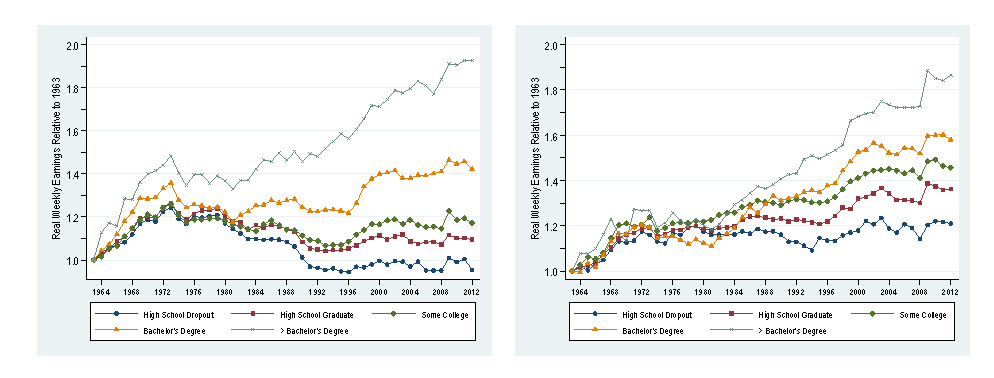
\includegraphics[keepaspectratio=true, scale=1, clip = true]{skills_premiumMW.pdf}
\caption{Change in Real Wage Levels of Full-Time Male (A) and female (B)
Workers by Education, 1963 - 2012, Autor 2014}
\label{fig:1.5}
\end{figure}

\end{document}

Plusieurs études ont montré que
les opportunités d'emploi aux États-Unis et dans de nombreux pays se sont fortement polarisées
au cours des deux dernières décennies. D'une part, les opportunités d'emploi se multiplient
tant dans les professions hautement qualifiées que dans les professions peu qualifiées. D'un autre côté, les opportunités d'emploi sont réduites dans les professions moyennement qualifiées.
  (emplois de cols blancs et de cols bleus). Étant donné que les tâches routinières sont souvent effectuées par des travailleurs moyennement qualifiés, cet exercice peut aider à expliquer le phénomène de polarisation des opportunités d'emploi.

%Cheaper computers lead to a rise in routine inputs 
Also show that as computers become cheaper, $w_N/w_R$ increases:  \begin{equation}\frac{\partial \ln (w_N/w_R) }{\partial \rho}=- \frac{1}{\beta}
\end{equation}


Several studies have shown that the structure of
job opportunities in the United States and many countries has sharply polarized
over the past two decades, with expanding job opportunities
in both high-skill, high-wage occupations and low-skill, low wage occupations, coupled with contracting opportunities in
middle-wage, middle-skill white-collar and blue-collar jobs.

This model allows to provide some explanation.  A leading
explanation focuses on the consequences of ongoing automation and offshoring of middle-skilled “routine” tasks that
were formerly performed primarily by workers with moderate
education (a high school diploma but less than a four-year college degree). 

Autor et al, find that a secular growth in non-routine interactive/cognitive occupations, and declining employment in routine-intensive occupations (but also a secular decline in non-routine manual tasks (a bit surporising given growth in low-skill services). They also find that computerization is associated with reduced labor input of routine manual and routine cognitive tasks and
increased labor input of nonroutine cognitive tasks.

In
this case, the wages paid to high skilled workers cannot exceed the rental price (per efficiency
unit) of the machine, and declines in the price of the machine (or increases in its efficiency)
will lower the price of skilled workers.  



%Routine tasks can be accomplished by following explicit rules. Problem-solving and communication activities are “nonroutine”
%tasks. 



The production function (\ref{autor}) implies that computer capital substitutes for workers in carrying out routine tasks. 
At the same time, a greater quantity of computers increase the marginal product of nonroutine tasks. Finally, notice that routine and nonroutine tasks are themselves imperfect
substitutes. 


\begin{equation}
\theta =(\frac{1-\beta}{\beta})^{1/\beta}
\end{equation}


\begin{equation}
\frac{w_N}{w_R}=\frac{\beta}{\1-\beta} (\frac{1-\beta}{\beta})^{1/\beta}
\end{equation}

Each worker $i$ is endowed with productivity $(n_i,r_i)$, where $r_i$ is the productivity in performing routine tasks while $n_i$ is the productivity in performing non-routine tasks. Assume $0<r_i,n_i \leq 1.$ The wage per efficiency unit of routine (respectively non-routine) task
input is $w_R$ (respectively $w_N$).


Workers must choose whether to supply routine or non-routine tasks. Workers choose to supply routine tasks iff \begin{equation} w_Rr_i \geq  w_Nn_i \end{equation} Given $w_R$ and $w_N$, it is possible to compute the labour supply of routine and non-routine inputs. For instance, the total supply of routine inputs is $g(w_R,w_N)=\sum_i (r_i) \cdot  I (w_Rr_i <  w_Nn_i) $ where $I$  is an indicator function. The  total supply of non-routine inputs is $h(w_R,w_N)=\sum_i (n_i) \cdot  I (w_Rr_i \leq  w_Nn_i) $. 

Because there is perfect substitutability of routine tasks
and computer capital, the wage per efficiency unit of routine task
input is pinned down by the price of computer capital


\bigskip

(3) Show that an increase in the wage premium $w_N/w_R$ will raise labor supply to the non-routine occupation: ''marginal" workers  reallocate labor supply from routine to nonroutine task input.  
Thus, when $\rho$ declines the increase in $\theta $ is met entirely by an increase of computer capital.



Answer: 
\begin{equation}
\frac{w_H}{w_L}= \frac{  (A_L L)^{\alpha}  (A_H)^{1-\alpha} (1-\alpha) H^{-\alpha}}{  (A_L)^{\alpha}  (A_H H)^{1-\alpha}\alpha L^{\alpha-1}}
\end{equation}


\begin{equation}
\frac{w_H}{w_L}= \frac{   (1-\alpha)  }{ \alpha }\frac{L}{H}
\end{equation}

The effect of technological progress: Technology progress (higher $A_L$ and $A_H$) has no effect on the college premium (the ratio $w_H/w_L$ but it raises both $w_L$ and $w_H$. Of course, if for instance  $A_L$ increases, one expects the marginal product of low skill labour $w_L$ to increase. Moreover, if $A_H$ increases, low skill benefits as well because in the Cobb-Douglas the marginal product of $L$ increases if $H$ becomes more productive. 

\medskip

The effect of H/L:  The model predicts that if $H/L$ increases, then the college premium decreases (which is not what we observed). The increase in the relative supply of high skilled worker will cause firms to reassign some ’tasks’ performed by low skilled workers to high skilled workers, thereby lowering the marginal productivity of high skilled workers and hence their relative wage. 

%https://www.oecd.org/skills/piaac/Skills%20volume%201%20(eng)--full%20v12--eBook%20(04%2011%202013).pdf 


 \begin{equation}
w_L= \frac{ \partial Y_t}{\partial L}= (A_L)^{\frac{\sigma -1}{\sigma }} L^{-1/\sigma} \left[ (A_L L)^{\frac{\sigma -1}{\sigma }}+(A_HH)^{\frac{\sigma -1}{%
\sigma }}\right] ^{\frac{1}{\sigma -1}}=
\end{equation}
 
 
  \begin{equation}
w_L=  (A_L)^{\frac{\sigma -1}{\sigma }} L^{-1/\sigma}  L^{1/\sigma} \left[ (A_L)^{\frac{\sigma -1}{\sigma }}+A_H^{\frac{\sigma -1}{%
\sigma }} (\frac{ H}{L})^{\frac{\sigma -1}{%
\sigma }}\right] ^{\frac{1}{\sigma -1}}=
\end{equation}



  \begin{equation}
w_L=  (A_L)^{\frac{\sigma -1}{\sigma }}  \left[ (A_L)^{\frac{\sigma -1}{\sigma }}+A_H^{\frac{\sigma -1}{%
\sigma }} (\frac{ H}{L})^{\frac{\sigma -1}{%
\sigma }}\right] ^{\frac{1}{\sigma -1}}=
\end{equation}


Answer:   \begin{equation}
\frac{w_H}{w_L}=   \frac{\frac{ \partial Y_t}{\partial H}}{\frac{ \partial Y_t}{\partial L}} = (\frac{A_H}{A_L})^{\frac{\sigma -1}{\sigma }} (\frac{H}{L})^{-1/\sigma}=
\end{equation}
\begin{center}


Everything else equal, as the fraction of skilled workers in the labor force increases, the wages of unskilled workers should increase. In other words, skilled and unskilled workers are ’Q-complements’: a greater quantity of the one increases the marginal product of the other.

%As the fraction of high skill workers in the labor force increases, the low skill wage should increase. This is an implication of imperfect substitution between high and low skill workers. An increase in the fraction (or relative supply) of high skill workers increases the demand for the services of low skill workers, pushing up their unit wage





Answer: This result is intuitive but will also turn out to be important: technological improvements of any sort will lead to higher wages for both skill groups in the canonical model (also following from q-complementary). Thus unless there is “technical regress,” the canonical model cannot account for declining (real) wages of a factor whose supply is not shifting outward.





Answer:   \begin{equation}
\frac{w_H}{w_L}=  (\frac{A_H}{A_L})^{\frac{\sigma -1}{\sigma }} (\frac{H}{L})^{-1/\sigma}=
\end{equation}
\begin{center}

There is a simple log linear relationship between the skill premium and the relative supply of skills as measured by H/L.

then an increase in t
 \bigskip
 \begin{equation}\label{ces}
Y_t=\left[ (A_L L)^{\frac{\sigma -1}{\sigma }}+(A_HH)^{\frac{\sigma -1}{%
\sigma }}\right] ^{\frac{\sigma }{\sigma -1}}
\end{equation}
 (2) Show that $w_L$ is increasing in both $A_H$ and $A_L$. Interpret this result.  In the data low skill workers  (particularly low skill male)
have experienced significant real earnings declines over the last decades. Can this simple model explain this decline ? 
\bigskip


(3) Show that the wage premium $w_H/w_L$ is decreasing in $H/L$ and, assuming that $\sigma>1$, is increasing in the skill-bias of technology $A_H/A_L$. Interpret this result. This model indicates that the wage premium is determined by a race between the increase in the supply of skills and skill-biased technical change, which increases the relative demand for high skills.  This model helps explain why the wage premium has increased in the 70s, when there was a deceleration in the growth of college relative supply .

\bigskip

\begin{center}
    
\textbf{Exercise 3} 
\end{center}

The previous model assumes that output is a function of skills ($H$ and $L$) and does not distinguish between workers’ skills and job tasks. In reality, the assignment of skills to tasks is determined in equilibrium by labor supplies,
technologies, and task demands. For example, college graduate may perform analytical tasks when computers are expensive, but may be replaced by computers when computers become cheaper. 


An alternative approach to (\ref{ces}) is given by  the task-based approach:  skills do not directly produce
output, but workers apply
their skills to tasks in exchange for wages. Assume the following production function:

\begin{equation}\label{autor}
    Y=(L_R+K)^{1-\beta}(L_N)^{\beta}
\end{equation}
$\beta \in (0,1)$, where $L_R$ and $L_N$ are routine and nonroutine labor inputs (‘‘tasks") and $K$ is computer capital, all measured in efficiency units.  Routine tasks can be accomplished by following explicit rules. Problem-solving and communication activities are “nonroutine”
tasks. One efficiency unit of computer capital costs $\rho$.  



The production function (\ref{autor}) implies that computer capital substitutes for workers in carrying out routine tasks. 
At the same time, a greater quantity of computers increase the marginal product of nonroutine tasks. Finally, notice that routine and nonroutine tasks are themselves imperfect
substitutes. 

Each worker $i$ is endowed with productivity $(n_i,r_i)$, where $r_i$ is the productivity in performing routine tasks while $n_i$ is the productivity in performing non-routine tasks. Assume $0<r_i,n_i \leq 1.$ The wage per efficiency unit of routine (respectively non-routine) task
input is $w_R$ (respectively $w_N$).


Workers must choose whether to supply routine or non-routine tasks. Workers choose to supply routine tasks iff \begin{equation} w_Rr_i \geq  w_Nn_i \end{equation} Given $w_R$ and $w_N$, it is possible to compute the labour supply of routine and non-routine inputs. For instance, the total supply of routine inputs is $g(w_R,w_N)=\sum_i (r_i) \cdot  I (w_Rr_i <  w_Nn_i) $ where $I$  is an indicator function. The  total supply of non-routine inputs is $h(w_R,w_N)=\sum_i (n_i) \cdot  I (w_Rr_i \leq  w_Nn_i) $. 

Because there is perfect substitutability of routine tasks
and computer capital, the wage per efficiency unit of routine task
input is pinned down by the price of computer capital

\begin{equation}
    w_R=\rho
\end{equation}
As a result, technological progress in the capital sector, which leads to a decline in the price of computers,  lowers $ w_R$.

Define the ratio of routine to non-routine inputs in production:  


\begin{equation}
    \theta \equiv \frac{L_R + K}{L_N} 
\end{equation}


\bigskip

(1) Solve the problem of the representative firm and find the demand of routine and non-routine inputs. Express these demands as a function of $\theta$.  Using the first order-condition with respect to $L_R$, find $\theta$ as a function of $\rho$.


\bigskip

(2) Since routine and non-routine tasks are complementary inputs, a decline in the price of computing power unambiguously increases the marginal productivity of workers engaged in non-routine tasks. Show that \begin{equation}\frac{\partial \ln w_N }{\partial \rho}= \frac{\beta -1}{\beta}<0
\end{equation}
 Also show that as computers become cheaper, the wage premium increases:  \begin{equation}\frac{\partial \ln (w_N/w_R) }{\partial \rho}=- \frac{1}{\beta}
\end{equation}

\bigskip

(3) Show that an increase in the wage premium $w_N/w_R$ will raise labor supply to the non-routine occupation: ''marginal" workers  reallocate labor supply from routine to nonroutine task input.  
Thus, when $\rho$ declines the increase in $\theta $ is met entirely by an increase of computer capital.


\begin{figure}[th]
\centering
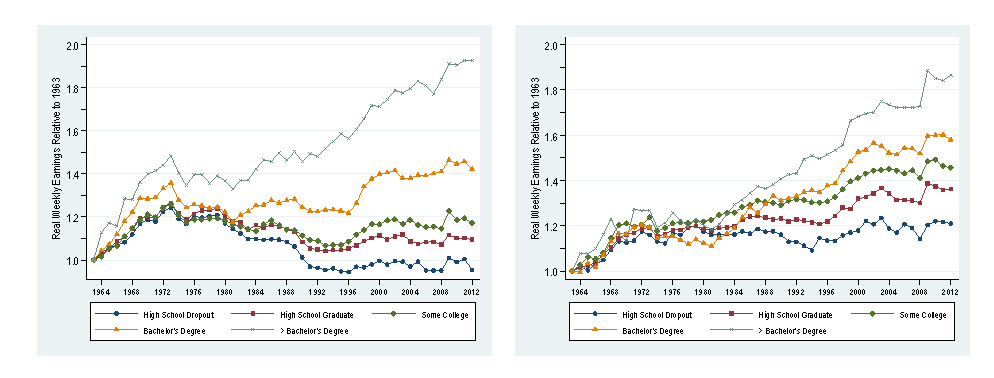
\includegraphics[keepaspectratio=true, scale=1.1, clip = true]{skills_premiumMW.pdf}
\caption{Change in Real Wage Levels of Full-Time Male (A) and female (B)
Workers by Education, 1963 - 2012, Autor 2014}
\label{fig:1.5}
\end{figure}

\end{document}

%w_Rr_i \geq  w_Nn_i
%the sum over the entire population  population endowments in ef��ciency units of routine and nonroutine tasks 


Workers are heterogenous: worker $i$ endowed with efficiencies (skills) given by  $E_i={r_i,n_1}$ where $n_i,r_i\in (0,1]$
Workers must choose whether to supply routine or non-routine tasks. Workers choose to supply routine tasks iff $w_Rr_i \geq  w_Nn_i$





Answer: We find that the saving rate is $s=\frac{\beta}{1+\beta}. $. 

Without capital markets, \begin{equation*} b^j_{t}=   sA (b^j_{t-1})^{\alpha}  \end{equation*}

and the steady state is $(sA)^{\frac{1}{1-\alpha}}$.

With perfect capital market, individual choose the optimal size of the activity

\begin{equation*}k^{\ast}=\arg \max_{k}  Ak^{\alpha} -Rk\end{equation*}



\begin{equation*}A\alpha k^{\alpha-1}=R\end{equation*}


\begin{equation*} k^{\ast}=(\frac{A\alpha}{R})^{1/(1-\alpha)}\end{equation*}


Profits

\begin{equation*} \pi=   A(k^{\ast})^{\alpha} -Rk^{\ast}\end{equation*}


\begin{equation*} m^j=   \pi + R b^j_{t-1} \end{equation*}

\begin{equation*} b^j_{t}=   s(\pi + R b^j_{t-1}) \end{equation*}

The transition is linear, with slope less than one. 

Without capital markets, \begin{equation*} b^j_{t}=   sA (b^j_{t-1})^{\alpha}  \end{equation*}

Suppose now that the production technology is: \begin{equation} y^j_t=A(k^j_t)^{\alpha} \ \  if \ \ k^j_t > \underline{k} \end{equation} 
 \begin{equation}  y^j_t=\underline{w} \ \ if \ \ k^j_t \leq \underline{k} \end{equation} 
Assume that R is not too big, so that profits $\pi$ are more than $\underline{w}$.  If capital markets are perfect, everybody chooses to use the CD technology


\begin{equation*} b^j_{t}=   s(\pi + R b^j_{t-1}) \end{equation*}

If  they are not perfect, we have 
 \begin{equation} b^j_{t}=   sA (b^j_{t-1})^{\alpha}  if \ \ k^j_t > \underline{k} \end{equation} 
 \begin{equation}  b^j_{t}=   s\underline{w} + (b^j_{t-1}) \ \ if \ \ k^j_t \leq \underline{k} \end{equation} 


Since the subsistence activity needs no capital, any capital that an individual owns is part of total income, but there is no interest earned on it, as capital markets are assumed to be absent.

\bigskip 

Expercise 2

 \begin{equation}
w_L= \frac{ \partial Y_t}{\partial L}= (A_L)^{\frac{\sigma -1}{\sigma }} L^{-1/\sigma} \left[ (A_L L)^{\frac{\sigma -1}{\sigma }}+(A_HH)^{\frac{\sigma -1}{%
\sigma }}\right] ^{\frac{1}{\sigma -1}}=
\end{equation}
 
 
  \begin{equation}
w_L=  (A_L)^{\frac{\sigma -1}{\sigma }} L^{-1/\sigma}  L^{1/\sigma} \left[ (A_L)^{\frac{\sigma -1}{\sigma }}+A_H^{\frac{\sigma -1}{%
\sigma }} (\frac{ H}{L})^{\frac{\sigma -1}{%
\sigma }}\right] ^{\frac{1}{\sigma -1}}=
\end{equation}



  \begin{equation}
w_L=  (A_L)^{\frac{\sigma -1}{\sigma }}  \left[ (A_L)^{\frac{\sigma -1}{\sigma }}+A_H^{\frac{\sigma -1}{%
\sigma }} (\frac{ H}{L})^{\frac{\sigma -1}{%
\sigma }}\right] ^{\frac{1}{\sigma -1}}=
\end{equation}

Everything else equal, as the fraction of skilled workers in the labor force increases, the wages of unskilled workers should increase. In other words, skilled and unskilled workers are ’Q-complements’: a greater quantity of the one increases the marginal product of the other.

%As the fraction of high skill workers in the labor force increases, the low skill wage should increase. This is an implication of imperfect substitution between high and low skill workers. An increase in the fraction (or relative supply) of high skill workers increases the demand for the services of low skill workers, pushing up their unit wage





Answer: This result is intuitive but will also turn out to be important: technological improvements of any sort will lead to higher wages for both skill groups in the canonical model (also following from q-complementary). Thus unless there is “technical regress,” the canonical model cannot account for declining (real) wages of a factor whose supply is not shifting outward.





Answer:   \begin{equation}
\frac{w_H}{w_L}=  (\frac{A_H}{A_L})^{\frac{\sigma -1}{\sigma }} (\frac{H}{L})^{-1/\sigma}=
\end{equation}
\begin{center}

There is a simple log linear relationship between the skill premium and the relative supply of skills as measured by H/L.

then an increase in the relative supply of high skilled worker will cause firms to reassign some ’tasks’ performed by low skilled workers to high skilled workers, thereby lowering the marginal productivity of high skilled workers and hence their relative wage. 

The downward sloping relationship between relative supply and the skill premium implies that if technology, in particular $AH/A_L$, had remained roughly constant over recent decades, the remarkable increase in the supply of skills shown in Fig. 1 would have led to a significant decline in the skill premium. The lack of such a decline is a key reason why economists believe that the first force in Tinbergen’s race—changes in technology increasing the demand for skills—must have also been important throughout the 20th century

Note that skill bias $(\frac{A_H}{A_L})$ increases the skill premium only if $\sigma >1$. That is, we need high skill and low skill workers are substitutes. When instead they are comp[lement ($\sigma <1$ )  a rise  in Ah/Al, cause their wages to fall (.  An intuitive way to see this is to consider a Leontief production function where high and low skilled workers are used in constant propor- tions in a competitive market. An increase in the supply of high skilled workers in this setting effectively creates “excess supply” for a given number of unskilled workers. The excess skilled workers will either bid down wages of other high skilled workers or will become unemployed (lowering average wages for skilled workers if zeros are counted). Since the broad consensus is that σ > 1, this case is generally thought to be unlikely.

 in the context of the substitution between college and non-college workers, a relatively high elasticity of substitution is both plausible and consistent with several studies. Most estimates put σ in this context to be somewhere between 1.4 and 2 



Answer:

\begin{equation}
\theta =(\frac{1-\beta}{\beta})^{1/\beta}
\end{equation}


\begin{equation}
\frac{w_N}{w_R}=\frac{\beta}{\1-\beta} (\frac{1-\beta}{\beta})^{1/\beta}
\end{equation}

\begin{figure}[th]
\centering
\includegraphics[keepaspectratio=true, scale=1.1, clip = true]{skills_premium.pdf}
\caption{comptabilit\'{e} de la croissance aux États-Unis (Jones, 2016)}
\label{fig:1.5}
\end{figure}

\end{document}

(3) Assume that over time there is a log linear increase in the demand for skills coming from technology: 
\begin{equation}
    ln(\frac{A_H}{A_L}) =\gamma_0 + \gamma_1  t
\end{equation}

where $t$ is calendar time.  Then, from  (\ref{ces2}) we obtain
\begin{equation}
    ln (\frac{w_H}{w_L}) = (\frac{\sigma -1}{\sigma}) \gamma_0 + (\frac{\sigma -1}{\sigma}) \gamma_1  t - \frac{1}{\sigma} ln (\frac{H}{L})
\end{equation}



%xplain why an increase of $\frac{A_H}{A_L}$ raises the college premium.   
\bigskip

Using data on wages and H and L from 1963 to 2008, Autor and Acemoglu (2011) estimated a linear regression and obtained the following OLS estimates:
%OLS regression of the compositionadjusted college/high school log weekly wage premium (Fig. 1) on a linear time trend
%and our measure of college/high school log relative supply (Fig. 2) for years 1963-1987. 


\begin{equation}
    ln (\frac{w_{H,t}}{w_{L,t}}) = constant + 0.016  t - 0.339 \ln (\frac{H_t}{L_t}) 
\end{equation}
Is the assumption $\sigma >1$ coherent with these estimates? 

%Argue that these estimates suggest that a plausible value for $\sigma$ is 2.9. 
%SInce $1/\sigma= 0.339$, suggesting $\sigma=2.9$. 


